\documentclass{article}
\usepackage[]{graphicx}
\usepackage[]{xcolor}
\usepackage{alltt}
\usepackage[left=2.3cm,right=2.8cm, top = 2.2cm, bottom = 3cm]{geometry}
\usepackage{amsmath}
\usepackage{amssymb}
\usepackage{natbib}
\PassOptionsToPackage{hyphens}{url}
\usepackage{url} 
\usepackage[disable]{todonotes}
\usepackage{multicol}
\usepackage{rotating}
\usepackage{booktabs}
\usepackage[colorlinks=false]{hyperref} 
\setlength{\parskip}{\baselineskip}%
\setlength{\parindent}{0pt}%

\bibliographystyle{apalike}

\newcommand{\red}{\color{red}}
\newcommand{\black}{\color{black}}
\newcommand{\blue}{\color{blue}}

\newcommand{\indented}{\setlength{\leftskip}{1cm}}
\newcommand{\notindented}{\setlength{\leftskip}{0cm}}

\begin{document}

%\black \textbf{Black: our comments}
%\red \textbf{Reviewer, not addressed}
%\blue \textbf{Reviewer, addressed} 


\black
We thank the reviewers for their feedback and thoughtful comments which we feel have helped improve the manuscript substantially. Please see our responses to the individual comments as well as explanations on the changes we have made to the manuscript below. 


\section{Reviewer \#1}

\blue
Bosse et al. discuss the important problem of forecast evaluation in the context of epidemiological models. They make a clear and compelling argument for the use of different variance-stabilising transformations to reduce the impact of variation in model outputs and data over several orders of magnitude, a consequence of the exponential nature of epidemic growth (with time-varying growth rate).

I only really have minor, hopefully constructive points to raise — overall I think this is a very nice piece of work that deserves to be published in close to its current form. My big picture and lower level comments and suggestions follow.

\black
Thank you for your kind words.

\blue
\subsection{Big picture}
\subsubsection{Proper scoring rules}
As noted by the authors, proper scoring rules are a commonly used concept in evaluating probabilistic predictions. While probably familiar to a reasonable fraction of readers, I think there is also likely a reasonable set of readers who are not aware of these or are only vaguely aware of them. For this reason I think a little more general background would help. For example on line 38 after the ‘report their true belief about nature’ another sentence or two along the lines of

“For example, some methods of ‘scoring’ probabilistic predictions can be ‘gamed’ in the sense that forecasters can do better by reporting a probability distribution different to their best estimate. A proper scoring rule ensures that the expected score when reporting a distribution Q, as evaluated under their actual best estimate of the probability distribution P, is best when Q = P. Thus a proper scoring rule encourages a forecaster to provide ‘honest’ predictions."

In addition, I suspect there are a few readers (such as myself!) who are more familiar with more ‘basic’ scores such as e.g. logarithmic score or arise (i.e. essentially the likelihood or related quantities). I spent a bit of time wondering about why these weren’t considered, especially as these avoid the scale issues at the centre of the present article. Such scores were only briefly considered in the discussion, in the second-to-last paragraph. I think it would be helpful to mention/emphasise up front some of these ‘classic’ scores that don’t have the same issues with scaling and then discuss why they aren’t used, e.g. due to ‘robustness’ or other issues (e.g. lack of full probability distributions from forecasts).

\black
We updated the paragraph, which now reads: 

\indented

Proper scoring rules are constructed such that they encourage honest forecasting and cannot be `gamed' or `cheated'. 
Assuming that the forecaster's actual best judgement corresponds to a predictive distribution $F$, a proper score is constructed such that under $F$, no other distribution $G$ yields a better expected score. Forecasters (anyone or anything that issues a forecast) are thus incentivised to report their true belief $F$ about the future. Common proper scoring rules are the logarithmic or log score \citep{goodRationalDecisions1952} or the continuous ranked probability score~\citep[CRPS,][]{gneitingStrictlyProperScoring2007}. The log score is the log-likelihood of the predictive density at the observed value and is scale-invariant under monotonous transformations. The log score does not suffer from the issues we address in this paper, but due to a number of reasons is not as widely used in fields such as weather forecasting or epidemiology (see e.g., \citealt{Johansson2019} for an exception). For example, the log score assigns particularly severe penalties to occasional misguided forecasts. This lack of robustness may limit its practical applicability \cite{bracherEvaluatingEpidemicForecasts2021}. Moreover, it is not easily applied to forecasts reported as samples or quantiles, as used in many recent disease forecasting efforts. 
For these reasons, the CRPS or its discrete equivalent, the ranked probability score~\citep[RPS,][]{funkAssessingPerformanceRealtime2019}, and the weighted interval score ~\citep[WIS,][]{bracherEvaluatingEpidemicForecasts2021} are more commonly used in epidemiology. 

\notindented

\blue
\subsubsection{Log vs other transformations}
The authors take the position that the log transformation is generally preferable for their use case, though they discuss and compare others. Relatedly, their arguments in terms of relative error also involve an essentially log-linear (i.e. log data + additive error) form which may be pragmatic but somewhat inelegant imo.

\black
In the theoretical part of the manuscript we simplify the equations a little bit by looking at the case of a single point forecast, rather than a probabilistic forecast that comes in the form of a predictive distribution. We feel this makes the discussion more intuitive. We want to emphasise that the log-linear error is really the error that is measured by the score, not the error model that would be assumed by any forecaster making a prediction. 


\blue
As the authors note, a particularly controversial issue for the log transformation is the issue of zero values. They take the standard pragmatic stance that we can use log (eps + y) instead of log y in such cases. Many communities e.g. econometrics are vehemently opposed to this, preferring e.g. quasi-Poisson regression and robust standard errors in the context of estimation. While not completely opposed to log (eps + y) myself (I have used it too!) it makes me a bit uncomfortable I still can’t help but feel that something along the lines of e.g. logarithmic/quasi-likelihood or deviance scores could be formulated that would be preferable to the log data transform. This would offer both automatic scaling and handling of zero values, in principle. However, I haven’t thought carefully enough to offer a concrete alternative and the log(eps + y) approach appears to work reasonably here. Instead, and in combination with the previous point, perhaps a bit more discussion of the potential alternatives based on quasi-likelihood-style functions rather than data transformations could be added?

\black
Thank you for raising this interesting point. The log score is indeed an alternative which is scale invariant under monotonic transformations. We mention this in the introduction and the the discussion and state that for the log score the question of which scale to evaluate forecasts on does not arise. In our understanding, a quasi-likelihood approach (as opposed to an actual likelihood approach as in the log score) may not actually be necessary as at least in theory full predictive distributions are to be evaluated. Developing further ideas based on some form of quasi-likelihood would likely require more in-depth investigation. In any case, developing these ideas would require more in-depth investigation and we feel this is beyond the scope of the current paper. 

\blue
\subsubsection{Observation and process models}
The interpretation in e.g. 2.2 appears to essentially assume a deterministic process model and additive error on the log scale (multiplicative on the natural scale). Although more of a motivating heuristic than strict assumption, a deterministic process model based on a mean will not in general be the same as a stochastic process model, right? Perhaps a further caveat that this is a fairly simplistic motivating tool might be useful?

Furthermore, why not assume that the model mean (say the output of the deterministic model) defines e.g. the mean of something like a Poisson distribution (probably in overdispersed/quasi form)? or negative binomial? The potential use of these distributions is considered in later sections in the context of motivating variance transforms, but then would again seem to motivate a (quasi-)likelihood-style score beyond the approximate transforms (though with pros and cons in terms of robustness, applicability in the presence of partial information).

\black
It is important to note that the equations in 2.2 do not refer to any particular model used by a forecaster or any model that was fit to data. Rather, we define the instantaneous growth rate for a single realised epidemic and then show that scoring forecasts for that on the log scale equates to scoring a forecast of the average growth rate according to this definition. The forecaster themselves who would make a forecast could assume any error model or model structure they like. 

\blue
\subsection{Specific suggestions}

I realised as I was about comment on some equations that none of the equations are numbered. It would probably be good to number them :-)

\black
This is a good point, we added numbers to all equations. 

\blue
The first equation (line 43) uses an unbolded indicator function which isn’t defined (this also appears in the same form in the third equation, line 99). The second equation in contrast uses bold and defines the indicator. The definition should be moved forward and a choice of bold or not made.

\black
We added the definition to equation according to your suggestion 1 and used bold throughout the manuscript consistently. 

\blue
I think the term ‘propriety’ (as in having the property of being proper) should either be explicitly defined or re-worded in terms of ‘being proper’.

\black
We reworded all occurrences of the term `propriety' in the text. 

\blue
No reference is provided for the approximate variance-stabilising properties of the square root transformation.

\black
We added a reference to the following book:
Dunn, P.K., Smyth, G.K.(2018). Generalized Linear Models With Examples in R. Germany: Springer New York, page 118. 





\blue
\section{Reviewer \#2}

\textbf{Summary}

This manuscript develops theory, interpretations, and intuition regarding evaluation metrics applied to strictly monotonic transformations of observations and forecasts, with focus on log, shifted log, sqrt, and shifted sqrt transformations, and details the application and impact of using a log1p transformation within an evaluation framework for COVID-19 forecasts.
The analysis is extensive and covers many facets of selecting and applying such transformations, providing great value. 

However, it
\begin{itemize}
    \item focuses on putting evaluations for different locations and times on an even scale, and does not directly answer the question of how to re-emphasize locations and times of import to forecast consumers, and
    \item the discussion of which locations and times forecasts consumers would want to emphasize seems incomplete.
\end{itemize}
The former point could be addressed by adding additional content regarding re-emphasis. The latter point could be addressed by studying what stakeholders want to emphasize and using that to make a recommendation for a particular transformation or transformation selection rule. Alternatively, both could be addressed simply by more explicitly and prominently noting that
\begin{itemize}
    \item when selecting a transformation, one should consider the desired emphasis, which is likely not an even scale for most/all predictions, and
    \item the “natural logarithm” / log1p selection is not meant as a recommendation but to enable demonstration.
\end{itemize}

\black

Thank you for your thorough and extensive comments. 
 
We added the following to the discussion to make our intentions clearer regarding the preferences of policy makers: 

\indented
In this paper, we did not make any particular assumptions about policy makers' priorities and preferences. Rather, we aimed to enable users to make an informed choice by showing how different transformations lead to different relative weights for the kinds of prediction errors forecast consumers may care about, such as absolute vs. relative errors or the size of penalties for over- vs. underprediction. In practice, engagement with decision makers is important to determine what their priorities are and how different ways to measure predictive importance should be weighed.

\notindented
It is important to note that changing the relative weight for different times and locations is one effect of the scoring forecasts on the log scale, but not necessarily the main point of the transformation. Rather, we do recommend to evaluate forecasts on the log scale as we believe the interpretation as a score of the exponential growth rate is meaningful in an epidemiological context. As stated explicitly in the manuscript, we moreover recommend to use this in complement to rather than as a replacement of the common evaluation on the ``natural scale''. Evaluators will then become aware of whether their results depend strongly on this decision and the implied weighting of different forecasting tasks.

Users who are explicitly concerned about the relative weights of different times and locations can e.g. find information in Figure 3 where we show how different forecast targets are emphasized by evaluation on the natural or log-transformed scale. A user could e.g. reproduce such a display with different values of the offset $a$ and choose $a$ such that the relative weighting of times and regions with high and low incidence correspond to their preferences. 

\blue
Additionally, any additional necessary/recommended elements of a scoring procedure should be noted more prominently (e.g., dealing with forecast missingness, outlying forecasts, outlying data, selecting a Box-Cox transformation, selecting a shift ($a$ value), etc.).

\black

To direct the readers' attention to the mentioned challenges already in the conceptual part of the paper we added the following paragraph to Section 2.4, which also contains a discussion of the choice of $a$:

\indented
We note that in the practical evaluation of operational forecasting systems  several additional challenges arise, which we do not study in detail. These concern e.g., the removal of outlying observations and forecasts and the handling of missing forecasts. The solutions we employed in practice are provided in Section 3.1.
\notindented

We added a paragraph on which kinds of transformations are permissible in Section 4 (see comments below). We agree that it would be useful to have a more thorough discussion of all the considerations involved in evaluating forecasts, but feel this is slightly beyond the scope of this paper. 

\blue
\subsection{Major comments}

``Natural logarithm'', log1p, and log($a + x$) are conflated in several places, despite the discussion in Section 2.4 noting that this is an important distinction. The terminology should not be overloaded. (E.g., L20 ``Applying the log transformation''.)

\black
We changed ``Applying the log transformation'' to ``Applying a transformation of log($x + 1$)'' in L20 (in the abstract). 

We slightly disagree with the notion that the terminology should not be overloaded. Not introducing another term for transformations of $\log_{e}(x + \varepsilon)$ makes the manuscript more readable and accessible to readers. In addition, our analyses suggest that adding a small offset doesn't make much of a difference in most practical applications. We nevertheless completely agree that this should be made clear to the reader and have added the following text: 

\indented
For conceptual clarity and to allow for a more in-depth discussion, we focus mostly on the natural logarithm as a particular transformation in the context of epidemic phenomena. We refer to this transformation as 'log-transformation' and to scores that have been computed from log-transformed forecasts and observations as scores 'on the log scale' (as opposed to scores 'on the natural scale', which involve no transformation). In the theoretical discussion in Section 2, 'log-transformation' and 'log scale' generally refer to a transformation of $\log_{e}(x)$. For practical applications (Section 3) we also use these terms to describe a transformation of $\log_{e}(x + \varepsilon)$ in order to keep the terminology and notation simple.

\notindented

\blue
L18:
\begin{itemize}
    \item ``relative error'' --- Is this what stakeholders want? Or does it overemphasize low steady periods too much?
    \item ``under the assumption of quadratic mean-variance relationship'' --- And do we expect/observe this sort of relationship in epidemiological surveillance data? This reads more like an arbitrary assumption that will be taken instead of something that is examined in the manuscript. (From Section 3.3 it seems like the answer is ``roughly but not entirely''.)
    \item These points might be more simply resolved simply by revising L15 ``motivate''.
\end{itemize}
\black 

We revised the word ``motivate'' in line 15. The sentence in the abstract now reads: 

\indented

Using the CRPS on log-transformed values as an example, we list three attractive properties: [...].

\notindented

We think the relative error is one option out of many that could be interesting to policy makers. 
Paireau et al. (2022, \url{https://www.pnas.org/doi/pdf/10.1073/pnas.2103302119}) for example specifically emphasize that in their work the use of MAPE is motivated by its
straightforward interpretation. But we agree that ultimately stakeholders need to decide for themselves what metrics they are interested in. As mentioned above, adjusting the offset before taking the logarithm is one way of dealing with periods of low counts, but this of course moves the interpretation of the score away from a score of the exponential growth rate. 

The assumption of a quadratic mean-variance relationship is not entirely arbitrary, but rather has a specific interpretation in the sense that it encodes the assumption that one can forecast the growth rate equally well regardless of the observed magnitude at the moment. In the manuscript, we state: 

\indented
The assumption of a quadratic mean-variance relationship is closely linked to the aspects discussed in Sections 2.1 and 2.2. It implies that relative errors have constant variance and can thus be meaningfully compared across different targets. Also, it arises naturally if we assume that our capacity to predict the epidemic growth rate does not depend on the expected outcome, i.e. does not depend on the current phase of the epidemic or the order of magnitude of current observations.

\notindented


\blue
L150: “it may be desirable” — Is it though? This seems unlikely. Stakeholders likely want to emphasize some locations and times over others, and would benefit from some rules about how to do so while maintaining propriety. (E.g., is scaling by some function of recent observations or the population size okay? Is scaling by the forecast or observed value okay? Or are we limited to monotonic transformations?)

\black
We think that while it is certainly not the only relevant approach, there is a case to be made for an evaluation which gives each forecasting target a similar weight. This is attractive if the goal of the evaluation is to find the best forecasting model for future use and if one assumes that the difficulty of the forecasting task is similar in different locations. Take for example two models that make independent forecasts for cases of COVID-19 in Germany, Luxembourg and Liechtenstein. CRPS scores on the natural scale would be dominated by the predictive performance in Germany. One model could be a lot better in Luxembourg and Liechtenstein and slightly worse in Germany and end up looking worse in terms of overall CRPS. However, it is unclear whether predictive performance in Germany really provides e.g. 100 times more information about how good a model is at predicting disease dynamics. If the question is which model to deploy in another location in the future, then it might be desirable to not have average scores be dominated by a single location. 

We have updated the paragraph as such: 

\indented
When evaluating models across sets of forecasting tasks, it may be desirable for each target to have a similar impact on the overall results. This could be motivated by the assumption that forecasts from different geographical units and time periods provide similar amounts of information about how well a forecaster performs. One would then like the resulting scores to be independent of the order of magnitude of the target to predict. CRPS values on the natural scale, however, typically scale with the order of magnitude of the quantity to be predicted. Average scores are then dominated by the results achieved for targets with high expected outcomes in a way that does not necessarily reflect the underlying predictive ability well.

\notindented

Regarding the question which transformations are permissible: 

Scaling by past observations is permissible (indeed taking the log is similar to scaling by the last value), as is scaling by the population size as mentioned in the discussion. There may of course be exceptions such as dividing by zero, but otherwise this just represents a monotonic transformation, which is unproblematic in terms of propriety. Scaling a forecast by the later observed value (as opposed to scaling by past observations) is generally not permissible as it disturbs propriety; see Lerch et al (2017, Statistical Science, preprint: \url{https://arxiv.org/abs/1512.09244}) on the closely related topic of weighting scores with a function of the observed value. Similarly, scaling a forecast by predictions made by other forecasters may break propriety, but we are unaware of existing theoretical arguments. Scaling scores, e.g. dividing a score by the mean score for other forecasters may be acceptable in most applied settings, but we are unsure about exactly when and how this could break propriety (as is the case for example when dividing by zero). 

To make this clearer in the text, we added the following paragraphs: 

\indented
A natural question is which other transformations could be applied and whether resulting scores remain (strictly) proper. In principle, any transformation function can be applied simultaneously to forecasts and observations as long as the definition of the transformation is independent of the forecasts and any quantities unknown at the time of forecasting, including the observed value. This simply corresponds to a re-definition of the forecasting target. However, applying non-invertible transformations leads to a loss in information conveyed by forecasts, which we consider undesirable. The resulting score will be proper, but it may not be strictly proper anymore (as forecasts differing from the forecaster's true belief on the original scale may be identical on the transformed scale). When using the CRPS or the WIS, it seems most appropriate to use only strictly monotonic transformations as otherwise the encoded notion of distance may become meaningless. If only strictly monotonic transformations are used, then transforming a forecaster's best belief on the original scale will correspond to their best belief on the transformed scale. This holds for both the log and square root transformations, as well as many others. 

Some other strictly monotonic transformations that can generally be applied prior to computing  the CRPS or WIS are scaling by the population size or scaling by past observations. The latter, as discussed in Section 4, is similar to applying a log-transformation, but corresponds to evaluating a forecast of multiplicative, rather than exponential growth rates. The arising issue of dividing by zero can again be solved by adding a small offset. This just represents a monotonic transformation and the remaining score is still strictly proper. Scaling a forecast by the later observed value (as opposed to scaling by past observations) is generally not permissible as it disturbs propriety (see \cite{lerchForecasterDilemmaExtreme2015} on the closely related topic of weighting scores with a function of the observed value). Similarly, scaling a forecast by predictions made by other forecasters may result in improper scores, but we are unaware of existing theoretical arguments. 

When applying a transformation, the order of the operations matters, and applying a transformation after scores have been computed generally does not guarantee that the score remains proper. In the case of log transforms, taking the logarithm of the scores, rather than scoring the log-transformed forecasts and data, results in an improper score. We illustrate this point using simulated data in Figure SI.1, where it can be seen that in the example overconfident models perform best in terms of the log WIS. Scaling scores (rather than forecasts and observations) by the mean score for other forecasters is closely related to the common practice of computing skill scores. While these are typically not technically proper \citep{gneitingStrictlyProperScoring2007}, their application is established practice and considered largely unproblematic.
\notindented



\blue
L166: “a negative binomial distribution with size parameter $\theta$” — Is this realistic? If so, what’s the interpretation epidemiologically?

\black
This is an illustrative example and is not meant to be completely realistic. Rather, the point is to illustrate that for observations which have a standard deviation that grows linearly with the mean, the log transformation can serve as a variance-stabilising transformation. However, negative binomial distributions are commonly used in the epidmeiological literature; see e.g., Section 3 of Meyer and Held (2017, \url{http://dx.doi.org/10.1214/14-AOAS743}). An epidemiological interpretation could be the following (see e.g. Funk, Abbott and Bracher \url{https://doi.org/10.1111/rssa.12974}):
\begin{itemize}
    \item For simplicity assume a generation time of one time interval (this could be relaxed).
    \item Each of the $Y_{t - 1}$ infected individuals at time $t - 1$  generates new infections at time $t$, with a reproduction number of $R_t$ and independent Poisson offspring distributions. Assuming independence across infecting individuals and given $R_t$ and $Y_{t - 1}$, $Y_t$ then follows a Poisson distribution with mean $R_t \times Y_{t - 1}$.
    \item We assume that $R_t$ is not fixed, but given by
    $$
    R_t = R_0 \times \theta_t
    $$
    where
    $$
    \theta \sim \text{Gamma}(\text{shape} = \psi, \text{rate} = \psi).
    $$
    \item This implies
    $$
    Y_t \mid Y_{t - 1} \sim \text{NegBin}(R_t \times Y_{t - 1}, \psi).
    $$
\end{itemize}
So a conditional negative binomial distribution with quadratic mean-variance relationship arises if we assume that a suitably distributed environmental factor $\theta_t$ modifies the reproductive number. While the assumption of this specific gamma distribution is arbitrary, a quadratic mean-variance relationship will also arise for other distributions of $\theta_t$.

This illustrates that a quadratic mean-variance relationship can arise from a simple yet not completely unreasonable renewal equation model.

\blue
Figure 3: is a geometric distribution realistic for epidemiological surveillance data?

\black
We agree that this is not a typical example we would expect to see in an epidemiological setting. It could happen in principle, but only in rather constructed cases. We still believe the example is valuable to illustrate the general point that the rankings between two forecasts can change even for a single observation. We added the following sentence:

\indented
We note that the chosen example involving a geometric forecast distribution is somewhat constructed; as shown in Section 3.4 and Figure 8A, rankings between models usually stay quite stable for a single forecast. .

\notindented


\blue
L236: “better able to illustrate the effects” — Why does this removal help illustrate the effects? Is such a removal procedure required to be able to apply this transformation approach at all? And if so, what are the requirements/considerations for such a removal procedure?

\black
We updated the paragraph as follows: 

\indented
In addition, we filtered out erroneous forecasts that were in extremely poor agreement with the observed data, as defined by any of the conditions listed in Table SI.2. Figure SI.6 shows the percentage of forecasts removed for each model. Those few (less than 0.2\%  of forecasts for each model) erroneous outlier forecasts had excessive influence on average scores and relative skill scores in a way that was not representative of normal model behaviour. We removed them here in order to better illustrate the effects of the log-transformation on scores that one would expect in a well-behaved scenario. In a regular forecast evaluation such erroneous forecasts should usually not be removed and would count towards overall model scores.

\notindented

\blue
L244: “pairwise comparisons” — The necessity of using an approach to handle missingness when combining evaluations should be noted more prominently from the beginning. The same applies to the outlier removal (if necessary) and a value selection.

\black
We added the following short paragraph to Section 2.4 to ensure these aspects are already mentioned in the conceptual part of the paper.

\indented
We note that in the practical evaluation of operational forecasting systems  several additional challenges arise, which we do not study in detail. These concern e.g., the removal of outlying observations and forecasts and the handling of missing forecasts. The solutions we employed in practice are provided in Section 3.1.

\notindented



\blue
Figure 4: The data (not) selected seems to obscure the key period of predicting the start of a case wave, as we expect the CRPS of log data to emphasize missed case increase predictions there more heavily than the natural scale. Deaths are not a substitute because they have access to a leading indicator and the same sort of misses may not be observed. The evaluations here may also miss some overshooting of the case peak. Which rules from Table SI.2 are coming into play and why? Is there a more complete alternative example?

\black
The data that was removed here was largely due to data revisions, not due to forecasts removed by the filtering on our part. 
We added the percentages of observed values in the main text and added the following two Figures in the SI to make that clearer. 

\begin{figure}[h!]
    \centering
    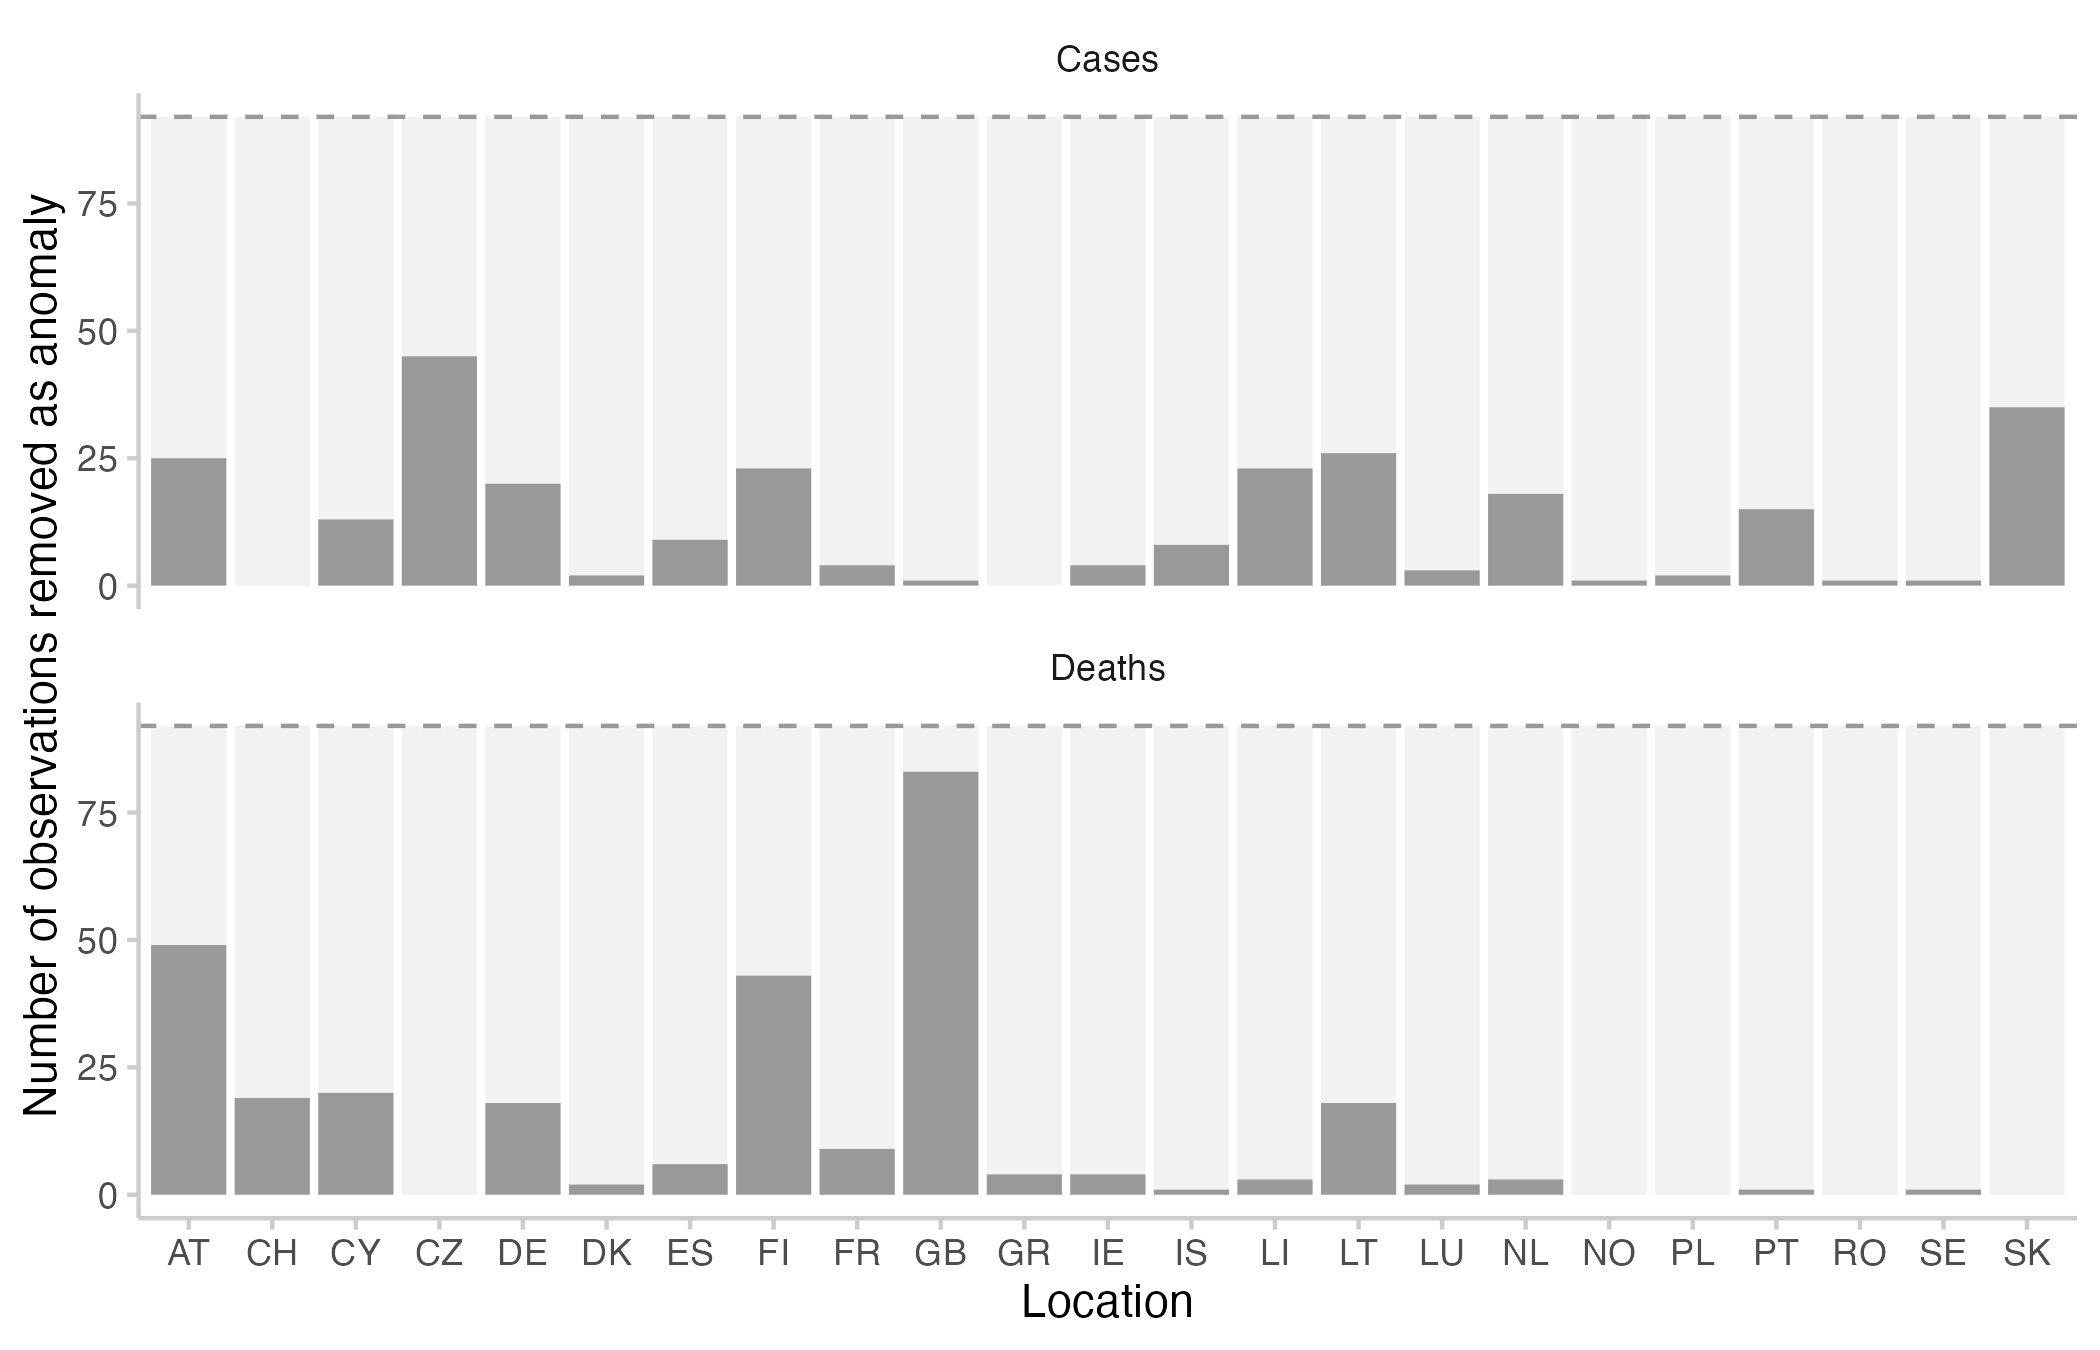
\includegraphics[width=0.49\textwidth]{output/figures/number-anomalies.png}
     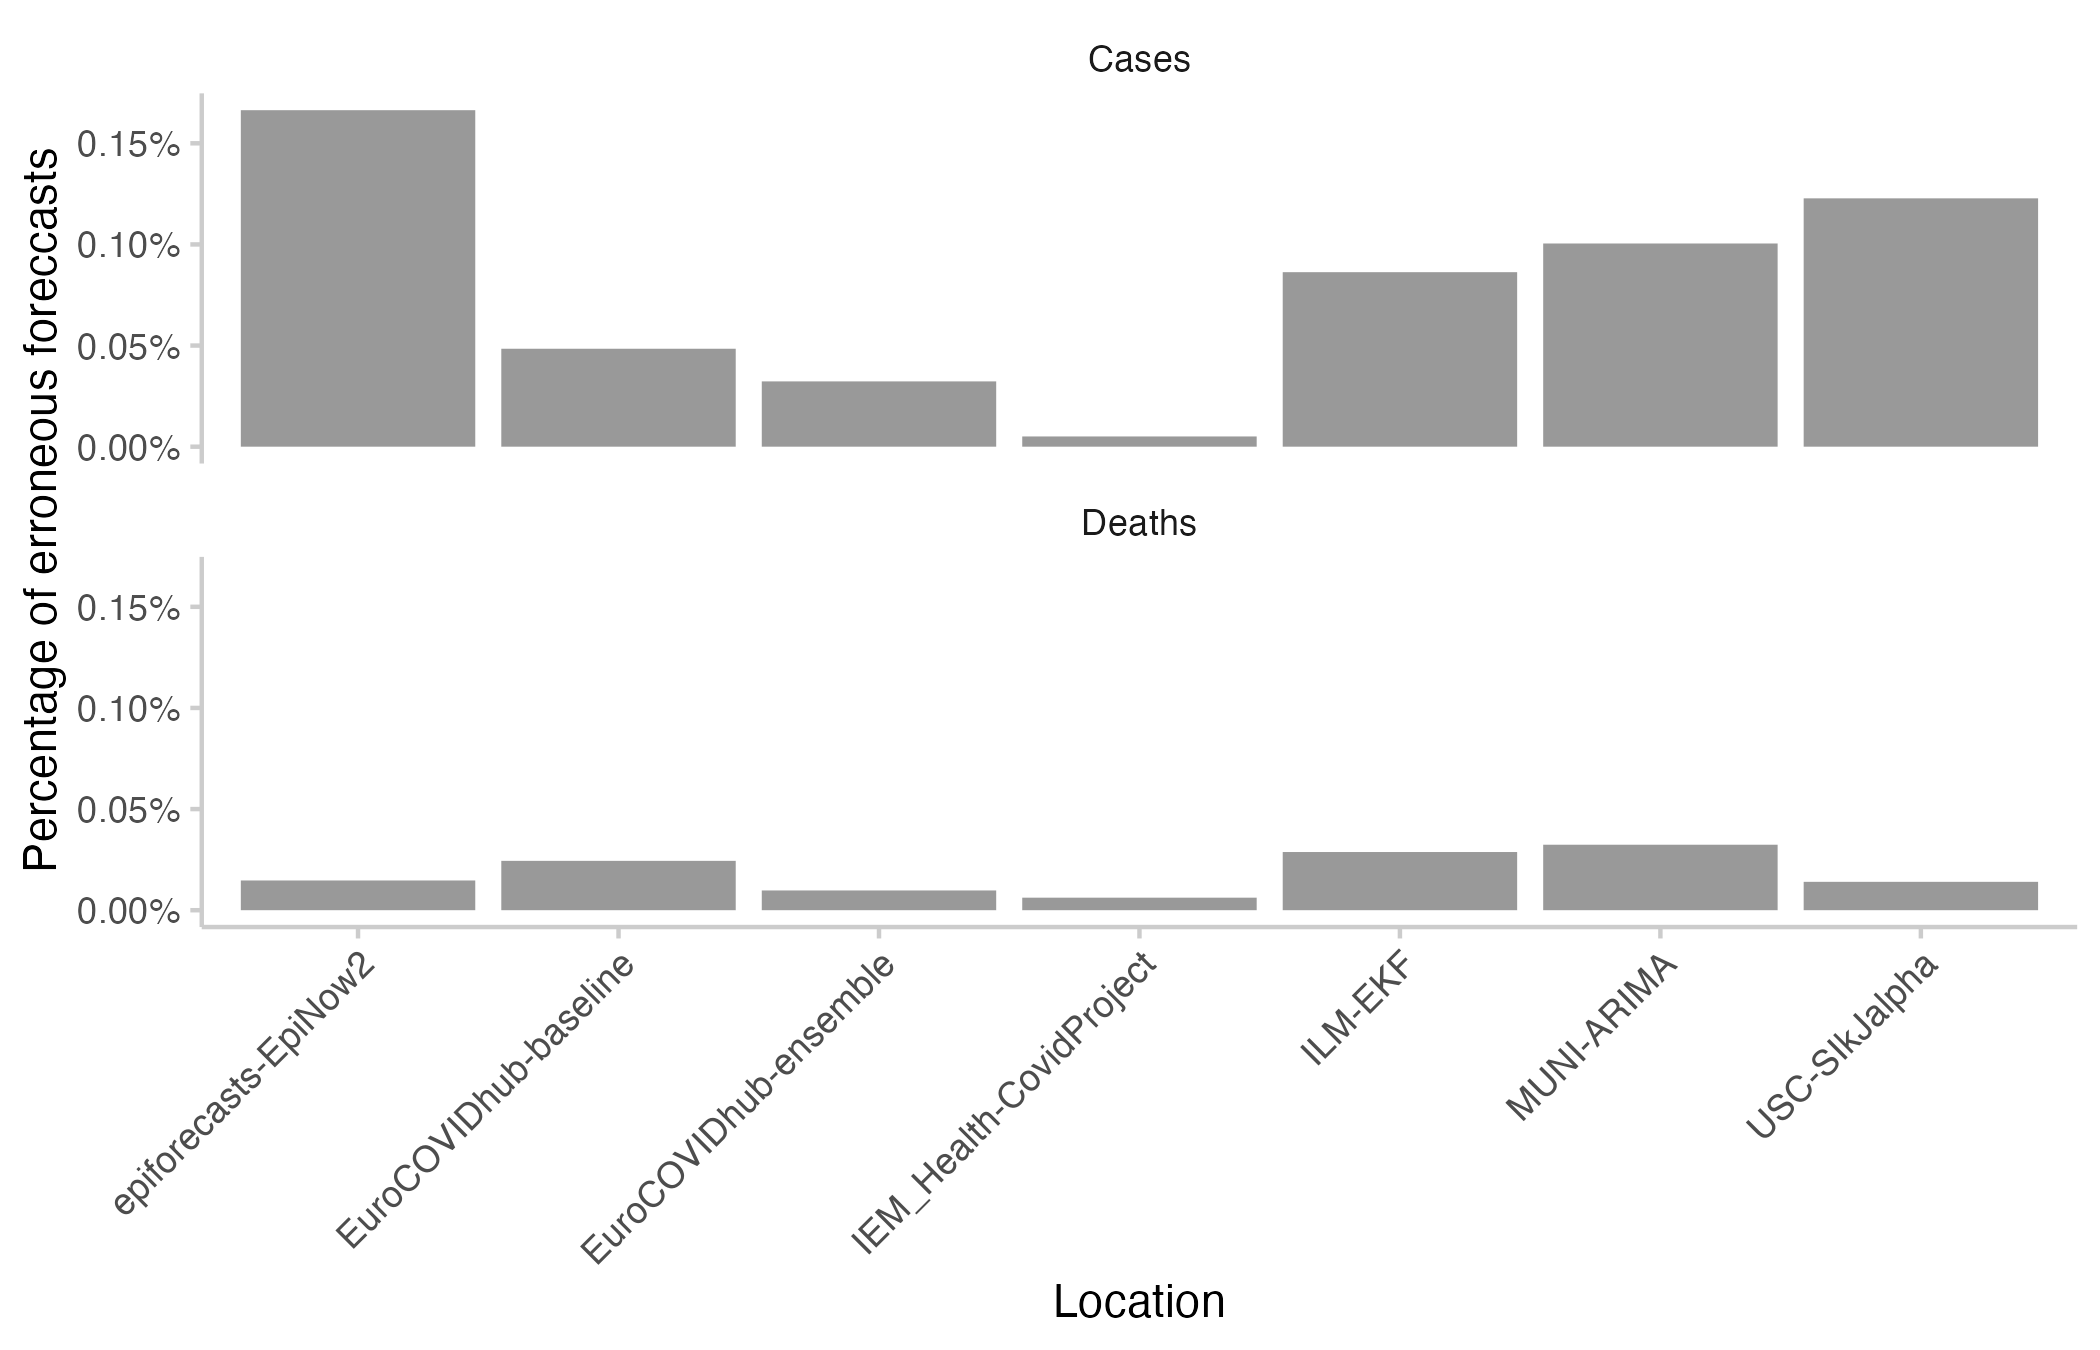
\includegraphics[width=0.49\textwidth]{output/figures/erroneous-forecasts.png}
     \caption{}
    \label{fig:number-anomalies}
\end{figure}


\blue
Table 1: The beta for cases and beta for deaths are both around 0.86 individually. But fit together they beta is 0.963; this appears due to trying to fit two different (difficulties of) tasks together that follow different trends, evident from the differing alpha values. A joint fit does not seem appropriate without allowing for a separate alpha per task type. The same thing can be said for the different horizons within cases\&deaths. The fits here seem to better support an argument for something between sd and log.

\black
We agree with the point, thank you for raising it. We removed the joint fit from the table. 

\blue
L279: “higher scores for smaller forecast targets” — This seems undesirable, given argument of Bracher et al. 2021a. Perhaps some forecast consumers would be interested in quality of forecasts for locations with lower activity (e.g., policymakers for smaller populations), but very unlikely would they want to prioritize less-active times in general over more-active times.  

\black 
We generally agree that giving higher weight to targets with lower incidences may be undesirable in many instances (one important exception is instances where times of low incidences are followed by upswings). Empirically, in our example, the additional weight given to smaller forecast targets on the log scale was rather small compared to the excessive weight given to larger forecast targets on the natural scale. However we agree that this is a trade-off. One potential avenue for future exploration might be a composite score that combines scores on the natural and on the log scale. 

\subsection{Minor comments}

\blue
L12 “over space and time” — Which do stakeholders care most about?

\black
We think that this is entirely up to the stakeholders and may depend on the setting. We hope that the reasoning and trade-offs involved become sufficiently clear throughout the remainder of the paper. 

\blue
L15 “log-transformed counts” — Immediately sounds problematic due to the possibility of 0 counts, without mention of a shift or threshold. Additionally, there is a truncated normal distribution in the mix; is it rounded to counts, or are these not all count data?

\black
We changed "log-transformed counts" to "log-transformed values" and updated the abstract to point out that we're applying a transformation of log($x + 1$) to our example data: 

\indented
Applying a transformation of log(x + 1) to data and forecasts from the European COVID-19 Forecast Hub

\notindented

The truncated normal distribution used as an example in Figure 2 is based directly on samples from the normal distribution, so here no rounding was applied. 

\blue
L23–L24 “more strongly emphasized”, “less severely penalized” — Could note that this is relative to evaluations on the natural scale (not relative to each other).

\black
Thank you for the suggestion. We updated the abstract as such: 

\indented
Situations in which models missed the beginning of upward swings are more strongly emphasised while failing to predict a downturn following a peak is less severely penalised when scoring transformed forecasts as opposed to untransformed ones.

\notindented

\blue
L24 “is only one” — Seems a bit too similar to “the only one”, “the only”, etc.

\black
We hope that the remainder makes it sufficiently clear that other transformations are possible. 

\blue
L46 “WIS is an approximation of the CRPS” — Is it an approximation of CRPS itself or some (2x?) scaling?

\black
The weighted interval score is a weighted sum of interval scores for the individual prediction intervals. When weighing the individual interval scores for the central $1 - \alpha$ prediction intervals by 
$w = \alpha / 2$ (which is generally standard), then the WIS converges exactly to the CRPS for an increasing number of equally spaced prediction intervals. For an illustration see Figure 2 in \cite{bracherEvaluatingEpidemicForecasts2021}.

\blue
L59 “strength” — The meaning of “strength” is nonintuitive without reading the citation and understanding the ties to multiplicative interventions on R and r (the latter of which seems unrealistic to achieve). Consider surrounding with quotes, explaining more/less, relating to growth per generation, etc.

\black
We updated the sentence to make this clearer. The new sentence is now: 

\indented
The reproduction number $R$ describes the number of people each infected person is expected to infect in turn (irrespective of the time between infections) and therefore is a measure of the strength of epidemic growth. The growth rate $r$ describes the speed of epidemic growth.

\notindented

\blue
L60: “immunity” $\xrightarrow{}$ “population immunity”?

\black
We changed this to "population immunity" as suggested. 

\blue
L69: This might benefit from a short justification (e.g.,
$\left| \frac{x_t e^{(r_t + \epsilon) \Delta t} - x_t e^{r_t \Delta t}}{x_t e^{(r_t - \epsilon) \Delta t} - x_t e^{r_t \Delta t}} \right| = e^{\epsilon\Delta t}$)

\black
This is a great suggestion, thank you. We updated the corresponding paragraph, which now reads: 

\indented
If case numbers are evolving based on an exponential process and the  modelling task revolves around estimating and forecasting the reproduction number or the corresponding growth rate, then evaluating forecasts based on the absolute distance between forecast and observed value penalises underprediction (of the reproduction number or growth rate) less than overprediction by the same amount. Consider a forecast that misses the correct growth rate by either $+\epsilon$ or $-\epsilon$:

\begin{equation}
\left| \frac{x_t e^{(r_t + \epsilon) \Delta t} - x_t e^{r_t \Delta t}}{x_t e^{(r_t - \epsilon) \Delta t} - x_t e^{r_t \Delta t}} \right| = e^{\epsilon\Delta t}
\end{equation}

For exponential processes errors on the observed value grow exponentially with the error on the estimated reproduction number or growth rate.

\notindented
\blue
L70: Clarify: is this suggesting to make the forecasting targets themselves the result of applying some standardized growth rate estimator to current+future observations around the desired time period?

\black 
Here we aren't suggesting a specific transformation yet, but rather just say that it would be desirable to score a forecast of the growth rate (regardless of how that can be achieved). Specific suggestions for how to achieve this (either by taking a log transformation or by using another transformation to obtain growth rates directly as mentioned in the Discussion) are discussed in more detail in the remainder of the text. We added the word 'conceptually' to the sentence to make this a bit clearer. 

\blue
L99: How are atoms at $\exp x = 0$ handled? How are observations of $y = 0$ handled?

\black
In the theoretical discussion in Section 2 we defined prediction targets to have strictly positive support, so these cases are excluded. In the later parts we follow the common strategy to add an offset before taking the logarithm. 

\blue

L127: “approximation of the absolute percentage error” — Raises a few questions:
\begin{itemize}
    \item If a relative error metric is desired, why not just divide CRPS/WIS by y then? (Propriety?)\\
    \black
Yes, dividing by the observed value generally disturbs propriety. This approach would correspond to weighting CRPS scores with weights depending on the observed value, and it has been shown that the resulting average scores are no longer proper; see Lerch et al (2017, Statistical Science, preprint: \url{https://arxiv.org/abs/1512.09244})
    \item \blue How does using a (shifted) log transform differ from dividing by (a constant plus) (a mean of) the most recent observation(s)?\\
    \black Like in the related arguments in the paper we address this question for the simpler case of the absolute error rather than CRPS. Using a shifted log transform corresponds to (in slight variation of equation (8))
    \begin{equation}
    |\varepsilon^*_t| = |\log (\hat{y_t} + a) - \log(y_t + a)| = \left|\log\left(\frac{\hat{y}_t + a}{y_t + a}\right) \right| \ \ \stackrel{\text{if } \hat{y}_t \ \approx \ y_t}{\approx} \ \ \left| \frac{\hat{y}_t + a}{y_t + a} - 1 \right| \ \ = \ \ \left| \frac{\hat{y}_t - y_t}{y_t + a} \right|.
    \end{equation}
    Dividing by the last observation plus a constant $a$, on the other hand, corresponds to
    \begin{equation}
    |\varepsilon^*_t| = \left|\frac{\hat{y}_t + a}{y_{t - 1} + a} - \frac{y_t + a}{y_{t - 1} + a} \right| = \ \ \left| \frac{\hat{y}_{t - 1} - y_t}{y_{t - 1} + a} \right|.
    \end{equation}
    If we interpret the denominator as an (inverse) weight for the different absolute errors, log transformation thus corresponds approximately equivalent to weighting with the inverse new observation $y_t$ (though better behaved in terms of the resulting incentives). Dividing by the previous value corresponds to weighting with the inverse preceding observation. As autocorrelation is typically strong in the time series we consider, this will yield similar, but not identical results.\\
    In terms of the epidemiological  interpretation, dividing by the last observed value can be interpreted as a score for a multiplicative, rather than an exponential growth rate. % We haven't investigated in detail how the two differ in their behaviour, but would expect them to yield mostly similar results. 
    \item \blue Is this desired? Though already discussed, seems like the major point of doubt here: are we at risk of overemphasizing very-low-activity periods and very-low-population states where standard-deviation-to- mean ratios are much higher?\\
    \black We agree that it may be an issue in practice that low-activity-periods could get overemphasised and therefore believe that an evaluation should show both scores on the natural scale as well as on the log scale. 
\end{itemize}







\blue

L127: As APE, RE, and SAPE are defined differently in other sources (e.g., with scaling factor in APE and SAPE, and with y in the denominator and no absolute value in RE), it may be helpful to also indicate sources for all three (e.g., that the RE definition is also in Gneiting, 2011).

\black
We added a reference to Gneiting (2011) for the relative error. SAPE is not defined in that paper, and we reference the paper by Flores (1986) instead. It seems that the earliest occurrence of the SAPE is due to a book by Armstrong (\textit{Long-range Forecasting: From Crystal Ball to Computer}, 1985); however, as we were unable to access the full text of this book we consider Flores (1986) the more helpful reference.

\blue

L138: “$\Bar{r}$ is” — Consider $\Bar{r}_t$ etc.

L146: “$\Bar{\hat{r}}$” — Should be $\hat{\Bar{r}}$, or consider $\hat{\Bar{r}}_t$.

\black
We applied the suggested changes.

\blue
L158 “delta method” — Delta method would seem to also require the distribution to be somewhat tightly distributed, concentrated within a nearly-linear region of the transformation function. But putting significant mass on a wider range of values would also mean having non-negligible mass on negative values if “approximately normal”; it would not make sense to apply the logarithm or sqrt transformations in these cases. So perhaps the “tightly distributed” assumption can be taken. But this seems a bit nonobvious and a justification/application of the delta method would be helpful here.

\black

This argument is a common justification for the choice of variance-stabilizing transformations, see e.g., the below excerpt from \textit{Generalized Linear Models With Examples in R} by Dunn and Smyth:
\begin{quote}
Suppose that $y$ has a mean-variance relationship defined by the function $V(\mu)$, with $\text{var}(y) = \phi V(\mu)$. Then, consider a transformation $y^* = h(y) \approx h(\mu) + h'(\mu)(y - \mu)$, from which it can be inferred that
$$
\text{var}(y^*) = \text{var}[h(y)] \approx h'(\mu)^2\text{var}(y).
$$
Hence, the transformation $y^* = h(y)$ will approximately stabilize the variance if $h'(\mu)$ is proportional to $\text{var}(y)^{-1/2} = V(\mu)^{-1/2}$. When $V(\mu) = \mu^2$ [...], the variance-stabilizing transformation is the logarithm, because then $h'(\mu) = 1/\mu$.  When $V(\mu) = \mu$, the variance-stabilizing transformation is the square root because $h'(\mu) = 1/\mu^{1/2}$.
\end{quote}

We added a reference to this source. We nonetheless agree with you that this approximation will work best if the distribution is tight and added a short remark to this regard.

The current paragraph reads: 

\indented

If the mean-variance relationship of the data-generating distribution is quadratic with $\sigma^2 = c \times \mu^2$, the natural logarithm can serve as the VST \citep{guerreroTimeseriesAnalysisSupported1993}. Denoting by $F_{\log}$ the predictive distribution for $\log(Y)$, we can use the delta method (a first-order Taylor approximation, see e.g., \citealt{Dunn2018}), to show that

\begin{equation}
\mathbb{E}_F[\text{CRPS}\{F_{\log}, \log(y)\}] \approx \frac{\sigma/\mu}{\sqrt{\pi}} 
= \frac{\sqrt{c}}{\sqrt{\pi}}
.
\end{equation}

The addition on ``tightly distributed'' probability mass reads

\indented
We note that while standard in the derivation of variance-stabilizing transformations, the application of the delta method in equations (16) and (17) requires the probability mass of $F$ to be tightly distributed. If this is not the case, the approximation may be less accurate.

\notindented



\blue
L159 — Need to discuss / spell out the point of the above calculation (— that it is the same for all $\mu$, when paired with the same $c$?).

\black
We added a sentence to make our point clearer: 

\indented
As $\sigma$ and $\mu$ are linked through the quadratic mean-variance relationship ($\sigma = \sqrt{c} \times \mu$), the expected CRPS stays constant regardless of the expeccted value of the data-generating distribution $\mu$. 

\notindented

\blue
L168: “grows with the variance” — May read like this a linear growth. Consider “grows with the standard deviation”.

\black
We have modified the sentence, which now reads: 

\indented
We see that when applying the CRPS on the natural scale, the expected CRPS grows monotonically as the variance of the predictive distribution (which is equal to the data-generating distribution for the ideal forecaster) increases.

\notindented
As the rest of the paragraph talks about the variance, we kept the word variance here as well. 

\blue

L180: “data-generating” — Consider “fitted”/“believed”.

\black
In this instance "data-generating" is correct, as this is about a general property of proper scoring rules. We changed the sentence slightly to make this clearer: 

\indented
We computed expected CRPS values  for three different distributions, assuming an ideal forecaster with predictive distribution equal to the true underlying (data-generating) distribution.


\notindented
\blue
L186: “incentivizes overconfident predictions” — Needs justifica- tion/citation/removal. This single example disproves propriety but doesn’t establish overconfidence as being encouraged in general.

\black
You are right. We removed that sentences as we do not have an analytical result on whether this holds in general. 

\blue
Figure 2: Were any zeros encountered for the negative binomial or Poisson distributions? Was a shifted log transformation used rather than an unshifted log transformation?

\black 
As indicated in the Figure legend ("Expected CRPS was computed on the natural scale (left), after applying a square-root transformation (middle), and after adding one and applying a log-transformation to the data (right)), we have added 1 before applying the log transformation to deal with zero values. 


\blue
L215: “is mainly driven” — Please add pointer to justification (e.g., Figure 7 / discussion).

\black
We added a reference to Figure 7. 

\blue
L231: “only include models which” — Consider “only include the 7 models that”

\black
Thank you for the suggestion, we edited the text accordingly. 

\blue
Figure 5 caption:
\begin{itemize}
    \item “logarithmic” — With what a values? (THe first link to Figure 5 is from before this information was stated.)
    \item “D: [. . . ] all individual scores” — of EuroCOVIDhub-ensemble or any of the 7 included systems?
    \item “relative change” — of what change in scores relative to what quantity?
\end{itemize}

\black
We have updated the caption, which now reads: 

\indented
Scores for two-week-ahead forecasts from the EuroCOVIDhub-ensemble (averaged across all forecast dates) for different locations, evaluated on the natural scale as well as after transforming counts by adding one and applying the natural logarithm. D: Corresponding boxplots of all individual scores of the EuroCOVIDhub-ensemble for two-week-ahead predictions. E: Boxplots for the relative change of scores for the EuroCOVIDhub-ensemble across forecast horizons. For any given forecast date and location, forecasts were made for four different forecast horizons, resulting in four scores. All scores were divided by the score for forecast horizon one. To enhance interpretability, the range of visible relative changes in scores (relative to horizon = 1) was restricted to [0.1, 10].

\notindented

\blue
L272: “with the standard deviation” — Also note here that this is for approximately normal data distributions?

\black 
We now remind the reader of this assumption by writing

\indented

As (under the simplifying assumption of normality, see Section \ref{sec:methods:vst}) the WIS/CRPS of an ideal forecaster scales with the standard deviation, a value of $\beta = 1$ would imply a quadratic median-variance relationship;

\notindented

\blue
L282: “independent” — Consider “linearly independent”.

\black
We changed the sentence accordingly.

\black

\blue
L288–290: What would stakeholders want this difference to be, and in
which direction? I would guess the sqrt would generally be preferable unless applying some extra transformation after the log to re-emphasize locations/times of interest.

\black
That likely depends on the exact purpose stakeholders have in mind. In many instances it is presumably not desirable to give large weight to smaller forecast targets, and one may therefore e.g. choose to use the sqrt transformation or a different one over the log transformation. On the other hand, in our example the log transformation only gives a little bit more weight to smaller forecast targets, which may be acceptable given that the log transformation has nice properties in terms of its interpretation in an epidemiological context. 

\blue
Figure 7 caption: “one score” — Consider clarifying that/whether there is potentially missingness here.

\black
We have updated the Figure caption to make it more easily understandable. It now reads: 

\indented
Correlations of rankings on the natural and logarithmic scale. A: Average Spearman rank correlation of scores for individual forecasts. For every individual target (defined by a combination of forecast date, target type, horizon, location), one score was obtained per model. Then, for every forecast target, the Spearman rank correlation was computed between scores on the natural scale and on the log scale for all the models that had made a forecast for that specific target. These individual rank correlations were then averaged across locations and time and are displayed stratified by horizon and target types, representing average accordance of model ranks for a single forecast target on the natural and on the log scale. B: Correlation between relative skill scores. For every forecast horizon and target type, a separate relative skill score was computed per model using pairwise comparisons, which is a measure of performance of a model relative to the others for a given horizon and target type that accounts for missing values. The plot shows the correlation between the relative skill scores on the natural vs. on the log scale, representing accordance of overall model performance as judged by scores on the natural and on the log scale.

\notindented

\blue
Figure 8: What is the meaning of the arrow colors? Initially it seems to match the direction, but there is also blue arrow pointing downward. If it is indicating the direction, please fix this and consider a third color for indicating unchanged ranks.

\black
The colour of the error indicates whether or not relative skill scores improved or deteriorated. We agree this was not at all clear and thank you for pointing this out. We updated the plot legend and added a more detailed explanation to the Figure legend: 

\indented
Red arrows indicate that the relative skill score deteriorated when moving from the natural to the log scale, green arrows indicate they improved.

\notindented

\blue
The WIS contribution decomposition suggests that an alternative baseline should be used based on differences in transformed data rather than differences in natural scale data. Or, alternatively, that the a value is too low to give reasonable comparisons (as data that is hard/impossible to distinguish from 0 on a plot on the natural scale corresponds with very high penalization of forecasts considering 0 as a possibility). This could (also) be noted in Figure SI.5’s caption.

\black
We agree that it would be interesting for the Forecast Hubs to explore baseline models based on transformed differences. However, in this application we aimed for coherence with previous analyses of the same data and thus included the baseline models created within the Forecast Hub in real time.

We also agree it is useful to flag the issues surrounding the selection of $a$ more prominently. We added the following sentence to the caption of Figure SI.5: 

\indented
One potential way to do deal with this could be to use a higher $a$ value when applying a transformation $\log(x + a)$, for example $a = 10$ instead of $a = 1$.

\notindented

We also added a similar sentence to a paragraph in the main text, which now reads: 

\indented

A related issue occurs when the predictive distribution has a large probability mass on zero (or on very small values), as this can translate into an excessively wide forecast in relative terms. This can be seen in Figure SI.5. Here, the dispersion component of the WIS is inflated for scores obtained after applying the natural logarithm because forecasts contained zero in its prediction intervals. To deal with this issue one could potentially choose to use a higher $a$ value when applying a transformation $\log(x + a)$, for example $a = 10$ instead of the $a = 1$ that we chose to use.

\notindented

\blue
L340: “convert [...] rate” — Please clarify. Does “multiplicative growth rate” refer to a setup with $\mathbb{E}[X_{t+k} | X_t] = X_t \theta^k$, or only a single step $\mathbb{E}[X_{t+\text{one step}} | X_t] = X_t \theta^k$? Does the proposed conversion apply to both, or only to the latter?

\blue
L341–342: “natural logarithm as a [. . . ] (VST)” — for what type of relevant distribution(s)?

\blue
L344: “take differences between forecasts on the log scale” — Clarify.

L345: “divide each forecast by the forecast” — Caveat about current forecast formats should be included here / in following sentences, without (one mention of) the idea about directly soliciting forecasts of week-on-week ratios in between.

\black
We updated the relevant paragraph which now reads:

\indented

We suggested using the natural logarithm as a variance-stabilising transformation (VST). This is appropriate for variables that are approximately normally distributed and have a quadratic mean-variance relationship with $\sigma^2 = c \times \mu^2$ (this is e.g. approximately true for the negative binomoial distribution and large $\mu$). Alternatively, the square-root transformation can be appropriate in the case of a Poisson distributed variable \citep{dunnGeneralizedLinearModels2018}. Other VST like the Box-Cox \citep{boxAnalysisTransformations1964} are conceivable as well.
If one is interested in multiplicative, rather than exponential growth rates, one could convert forecasts into forecasts for the multiplicative growth rate by dividing numbers by the last value that was observed at the time the forecast was made. Forecasters would then implicitly predict a separate multiplicative growth rate from today to horizon 1, 2, etc. 
Instead of dividing by the last observed value, another promising transformation would be to divide each forecast by the forecast of the previous week (and analogously for observations), in order to obtain forecasts for week-to-week growth rates. Alternatively, one could also take first differences of values on the log scale. This approach would be akin to evaluating the shape of the predicted trajectory against the shape of the observed trajectory \citep[for a different approach to evaluating the shape of a forecast, see][]{srivastavaShapebasedEvaluationEpidemic2022}. Dividing values by the previous value, unfortunately, is not feasible under the current quantile-based format of the Forecast Hubs, as the growth rate of the $\alpha$-quantile may be different from the $\alpha$-quantile of the growth-rate. However, it may be an interesting approach if predictive samples are available or if quantiles for weekwise growth rates have been collected. 

\notindented

\blue
L366: “[...] settings” — (to standardize between measurements, then
could potentially scale by importance to stakeholders)

\black
We slightly adapted the text to make this point clearer: 

\indented
It is possible to go beyond choosing a single transformation by constructing composite scores as a weighted sum of scores based on different transformations. This would make it possible to create custom scores and allow forecast consumers to choose and assign explicit weights to different qualities of the forecasts they might care about.

\notindented


\blue
Figure SI.2: Would benefit from some more discussion, and perhaps a plot of slightly different quantities. E.g., to select an appropriate value of a, it seems like a common goal would be to deprioritize errors around values of x low enough that we expect there to be primarily noise rather than signal or that are not of concern to policymakers. For count data, this likely includes the values 0 - -10 in any circumstances; how far beyond 10 this range extends depends on the range of realistic growth rates, the forecast horizon, and cleanliness of the data. To assist in this decision, it seems like a similar plot of the evaluations of a particular absolute and/or relative error might be useful, or discussion of how to read it from the current plot. E.g., to illustrate that the same relative error is penalized roughly the same for all the plotted values of a for values of x above 50, but quite differently for $a = 10$ vs. $a = 0.1$ for values of x near 1.

\black

We added some more explanation to the caption of Figure SI.2. This makes the trade-off involved in choosing a suitable $a$ value clearer, without prescribing a 'correct' solution. 

\indented
For a given solid line, the dashed line of the same colour marks the x-value that  is equal to 5 times the corresponding offset. It can be seen that for $a$ values smaller than one fifth of the transformed quantity, the effect of adding an offset is generally small. When choosing a suitable $a$, the trade-off is between staying close to the interpretation of a pure log-transformation (choosing a small $a$) and not giving excessive weights to small observations (by choosing a larger $a$, see Figure 3).

\notindented

\blue
Figure SI.7:
\begin{itemize}
    \item Also specify sorting variable\&direction on x axis. (Would a point plot vs. the sorting variable be more informative?)
    \item Very informative figure, promote to main text? Also would like to see for different “parts” of an epidemic (e.g., steady low periods, increases, peaks/plateaus, decreases). Deaths figures suggest that balancing scores between locations can be tricky, and both cases and deaths suggests that the investigated transformations can’t do this exactly.
\end{itemize}

\black
We added a statement to the legend "Locations are sorted according to the mean observed value in that location." We also followed your suggestion to make this a main figure. 

We would expect that one could find a value for a that would eventually yield a more or less flat line, but we haven't investigated this in practice. 

\blue
\subsubsection{Typographical}
\blue
L96: “transformtation” $\xrightarrow{}$ “transformation”

Figure 2 caption: “CRPS values where computed” $\xrightarrow{}$ “[...] were computed”

L192: “does however influences” $\xrightarrow{}$ “does however influence”

L249: use two backticks on the left and two single quotes on the right in LaTeX code for the quoting here

Figure 5: “Loaction” → “Location”

Figure SI.7: “Loaction” → “Location”

\black
Thank you very much for pointing these errors out. We have corrected them. 


\blue
In several places, e.g., L201, there are links to SI material, when clicked, that instead redirect to main text figures.

\black
We're not sure why this happens and apologise for the confusion. We're also admittedly not sure how to fix this, but expect this will be dealt with during final typesetting. 

















\blue
\section{Reviewer \#3}

In this manuscript the authors investigate how common scoring rules for probabilistic forecasts can be adjusted by transforming observed data and forecast predictions prior to scoring. They provide three clear motivations for applying such transformations prior to scoring, assess the implications of different transformations in great detail, and evaluate the effects of these transformations using real-world COVID-19 forecasts obtained from the European Forecast Hub. Approaches that can help us improve how we measure the utility of epidemic forecasts for decision-makers are definitely needed. This is a very nice and timely contribution to epidemic forecast evaluation, and I only have a few comments.

\black
Thank you for your kind words. 

\blue
1. Line 96, typo: "log-transformtation".

\black
We corrected the typo

\blue
2. Figure 3: out of curiosity, do the rankings of forecasts A and B first switch at the same observed value (somewhere around 7?) in both panels? Zooming in, it looks as though maybe the switch occurs very slightly earlier for the log-transformed scoring.

\black
On the natural scale, the switch happens between 6.5 and 6.6 and on the log scale between 6.2 and 6.3. 

\blue
3. Section 3.2, page 9: remarks concerning Figure 4 refer to months (e.g., May, July) but it's a little difficult to relate them to the figure, because the x-axis only has 6-month breaks and spans two years, so it isn't immediately apparent which year (or both?) the reader should focus on. That being said, it's great to see how the log-transformation yields similar scores when the forecasts miss peaks and troughs.

\black
That's a good point, we made the references in the text clearer and added years. 

\blue
4. Line 281: missing closing parenthesis, "(or $\beta_{\sqrt{}} = 0$, respectively".

\black
We corrected the typo

\blue
5. Figure 7: I can appreciate that the correlation between the natural and logarithmic scores decreases over the forecast horizon, as the absolute forecast error grows. But I found panel B more challenging to interpret. I gather the key message is that model rankings are quite consistent between the natural and log scales (panel A) even though the absolute scores differ markedly between the two scales — an effect that increases over the forecast horizon (panel B). Perhaps adding a sentence to this effect in the accompanying text (lines 292-295) would help other readers to avoid my confusion.

\black
We adapted the text and hopefully made it more clear: 

For \textit{individual} forecasts, rankings between models for single forecasts are mostly preserved, with differences increasing across forecast horizons (see Figure \ref{fig:HUB-cors}A). While rankings between forecasters remain similar for a single forecast, this is not true anymore when looking at rankings obtained after averaging scores across multiple forecasts made at different times or in different locations. As discussed earlier, scores on the natural and on the log scale penalise errors very differently, e.g. when looking at performance during peaks or troughs. When evaluating performance \textit{averaged across} different forecasts and forecast targets, relative skill scores of the models therefore change considerably.


\blue
6. Line 296, typo: "Figure Figure 8 shows ...".

\black
We corrected the typo

\blue
7. Section 3.4, page 14 and Figure 8: it's a welcome outcome that the Hub ensemble forecast remained the top model, given that the log-transformation clearly affects the individual model rankings. Presumably it would be reasonable to expect that ensemble forecasts for other regions, pathogens, etc, should be the best (or near-best) model when using log-transformed case counts?

\black
While more research is needed to conclude this with more confidence, we generally agree with the statement. We would also expect ensemble forecasts to do well (as they have done in the post) regardless of whether they are evaluated on the log or on the natural scale. 

\blue
8. Lines 327-329: "A potential downside is that forecast evaluation is unreliable in situations where observed values are zero or very small."

I feel there's an argument to be made here that rather than being a potential limitations, it could be considered an accurate reflection of the inherent uncertainty about the future course of an epidemic when case numbers are very small. This transformation also provides a valuable benefit in these situations, as the authors note a few sentences later: "It also gives higher weight to another type of situation one may care about, namely one in which numbers start to rise from a previously low level". This neatly illustrates the importance (as highlighted by the authors in this manuscript) of using multiple scoring rules to evaluate and compare forecasts.

\black
We added a sentence: 

One could argue that this correctly reflect inherent uncertainty about the future course of an epidemic when numbers are small. Users nevertheless need to be aware that this can pose issues in practice. 

\blue

9. Table SI.2, "Criteria for removing forecasts": forecasts were removed if their median prediction differed greatly from the true value. This should probably be mentioned in the manuscript text, somewhere around line 235 (where Table SI.2 is referenced), to notify the reader that the definition of "erroneous forecasts" includes forecasts that are in extremely poor agreement with the ground truth. Otherwise, I feel that "erroneous" may be open to misinterpretation (e.g., only removing forecasts that predicted negative counts, NaN values, etc).

\black
This is a good point. We changed the sentence to 

In addition, we filtered out a small number of erroneous forecasts that were in extremely poor agreement with the observed data, as defined by any of the conditions listed in Table SI.2. 







\clearpage
\bibliography{log-or-not-v2.bib, log-or-not.bib, software.bib}

\end{document}
